\documentclass[12pt]{article}
\usepackage{latexsym}
\usepackage{amsmath, setspace, amssymb}
\usepackage{graphicx}
\usepackage{fancyhdr}
\usepackage{enumerate}
\usepackage{listings}
\usepackage{bbold}
\usepackage{cancel}
\usepackage{tipa}
\usepackage{multirow}
\usepackage{multicol}
\usepackage{url}
\usepackage{MnSymbol}
\usepackage{subcaption}
\usepackage{caption}
\usepackage{color}
\usepackage{pgfplots}
\usepackage[section]{placeins}

\pdfpagewidth 8.5in
\pdfpageheight 11in

\setlength\textwidth{7.0in}
\setlength\oddsidemargin{-0.25in}
\setlength\evensidemargin{-0.25in}
\setlength{\parindent}{0pt}

\setlength\textheight{8.75in}
\setlength\topmargin{-0.25in}
\setlength\headheight{0in}
\setlength\headsep{.3in}

\newcommand{\vb}[1]{\vec{\bold{#1}}}
\newcommand{\pp}[2]{\begin{pmatrix} #1 \\#2 \end{pmatrix}}
\newcommand{\ppp}[3]{\begin{pmatrix} #1 \\#2\\ #3 \end{pmatrix}}
\newcommand{\vv}[2]{\begin{bmatrix} #1 \\#2 \end{bmatrix}}
\newcommand{\vvv}[3]{\begin{bmatrix} #1 \\#2 \\#3 \end{bmatrix}}
\newcommand{\limit}[2]{\lim_{#1\to#2}}
\newcommand{\RR}{$\mathbb{R}$}
\newcommand{\R}[1]{\mathbb{R}^{#1}}
\newcommand{\st}{\text{ s.t. }}
\newcommand{\qmatrix}[4]{\begin{bmatrix}#1&#2\\#3&#4\end{bmatrix}}
\newcommand{\beeqn}{\begin{eqnarray*}}
\newcommand{\eeqn}{\end{eqnarray*}}
\newcommand{\ban}[1]{ \begin{align*}#1\end{align*} }
\newcommand{\ba}[1]{ \begin{align}#1\end{align} }
\newcommand{\inv}[1]{{#1}^{-1}}
\newcommand{\beeqnn}{\begin{eqnarray}}
\newcommand{\eeqnn}{\end{eqnarray}}
\newcommand{\no}{\noindent}
\newcommand{\mathbox}[1]{\ban{\boxed{#1}}}
\newcommand{\grad}{\vec \nabla}
\newcommand{\pd}[2]{\frac{\partial#1}{\partial#2}}
\newcommand{\deriv}[2]{\frac{d#1}{d#2}}
\newcommand{\mathsym}[1]{{}}
\newcommand{\unicode}[1]{{}}
\newcommand{\benum}{\begin{enumerate}[a)]}
\newcommand{\eenum}{\end{enumerate}}
\newcommand{\corr}[1]{\left<#1\right>}
\newcommand{\noor}[1]{:#1:}
\newcommand{\ket}[1]{\left|#1\right>}
\newcommand{\Lagr}{\mathcal L}
\newcommand{\sq}{\flushright$\square$\flushleft}
\newcommand{\reef}[1]{(\ref{#1})}
\newcommand{\Sf}{\mathcal S}
\newcommand{\Res}{\text{Res}}

\pagestyle{fancy}
\lhead{Smunch}
\rhead{Modeling}

\begin{document}

\thispagestyle{empty}

\begin{center}

\large Smunch\\
Internship 2017 (summer)\\
\vspace{0.5cm}
\normalsize 
Wednesday July 12 \hfill Noah M. Schumacher\\
\vspace{0.25cm}
\Large {\textbf{Order Predicting}}\normalsize
\end{center}

This document will go over the factors that lead to a user ordering Smunch or not. It will detail possible approaches for using collected data to predict:
\begin{enumerate}
  \item If a user will order on a certain day.
  \item How many orders a company will place on a given day
  \item How many orders a certain restaurant can expect on a given day.
\end{enumerate}
It will also explore the timing of orders. By this I mean at what time a company historically placed 90\% of its orders. From this historical data we can predict when 90\% has been placed. Hopefully this information will provide insights to number of total orders placed and can be incorporated in the prediction modeling.\\

%%%%%%%%%%%%%%%%%%%%%%% Section 1 %%%%%%%%%%%%%%%%%%%%%%%%%%%%
\section{Preliminaries: User Factors}

\begin{table}[!htb]
\begin{center}
\textbf{User order factors.} \\ [1.2ex]

 \begin{tabular}{||c c c||} 
 \hline
 \textbf{Factor} & \textbf{Strength} &\textbf{Description} \\ [0.7ex] 
 \hline\hline
 Restaurant & ***** & The food offered on given day (ratings, type, ...). \\ [1ex]
 \hline
 Delivery Time & ** & When the food is expected to be delivered. \\ [1ex]
 \hline
 Friends/Coworker Orders & **** & If others in office are ordering. \\ [1ex]
 \hline
 Weather & *** & Weather forecast. \\ [1ex]
 \hline
 Day of the Week & **** & What day of the week it is. \\ [1ex]
 \hline
 Age & ** & Age of User. \\ [1ex]
\hline
 Company location & **** & Company close to good food? \\ [1ex]
\hline
Salary & ** & Salary of User. \\ [1ex]
\hline
Hours per day& * & How long User works per day. \\ [1ex]
\hline
Order Trend & ***** & Trend of previous User orders. \\ [1ex]
\hline
Rating& *** & Users recent and/or overall ratings. \\ [1ex]
\hline
Type of Job& *** & Users job category. (sales, dev, ops, ...) \\ [1ex]
\hline
\end{tabular}
\caption{User order factors table showing possible parameters/variables and guessed weighting strength}
\label{}
\end{center}
\end{table}

\vspace{0.25cm}

     From these factors their are two possible routes for determining expected order. Use of a multiple regression algorithm (most likely linear) will take in these weighted independent variables and produce an expected total order count from a company. Or, a decision tree which would ultimately lead to a yes or no decision for the User ordering or not.
     I think that using a multiple regression model to predict the total company orders would be the best method. To start off only around 5 factors will be necessary for individual user predictions. I believe the five most important factors, that continuously update are:

\begin{itemize}
  \item Restaurant (companies previous order totals from restaurant)
  \item Day of the Week
  \item Rating (companies previous order totals from restaurants with given rating)
  \item Weather
  \item Delivery Time
\end{itemize}
\vspace{0.25cm}

Note: \small I mention continuously update because some of the factors might not play a different role everyday but are a one time factor that underlines a trend; e.g. A company location might be in an area with limited food options which leads to a higher number of employees using Smunch and also a higher density of orders per day. But this factor does not continuously change and therefore is captured in the other relevant information, such has order trend.

\vspace{.5cm}
Difficulties:\\
    While the idea of a regression model seems easy we run into problems because these factors iterate and update in all different ways. So instead a of a unified regression such as the one below:
    
\ban{
Order Percentage(x_1, x_2, x_3, x_4, x_5) = \beta_0 + \beta_1 x_1 + \beta_2 x_2 + \beta_3 x_3 + \beta_4 x_4 + \beta_5 x_5
}

\vspace{0.25cm}
Where the $\beta$ parameters are the partial regression coefficients and $x$'s are the predictor variables. It might be more meaningful to gather data independently and then combine based on the given parameters for a day. Perhaps this is best explained in an example.\\

Say we are given the table below \label{table:1}. From the data we can gain insights to the future week by taking various trends from previous data like so.


\begin{table}[!htb]
\center
\begin{tabular}{||c c c c c||}
 \hline
 Observation & DayofWeek & Restaurant & RestRating & CompanyOrders  \\ [0.5ex] 
 \hline\hline
 1 & Mon & Rest1 & 4 & 20 \\ 
 2 & Tue & Rest2 & 2 & 12 \\
 3 & Wed & Rest3 & 3 & 48 \\
 4 & Thu & Rest4 & 4 & 10 \\
 5 & Fri & Rest5 & 3 & 23 \\
 6 & Mon & Rest6 & 5 & 25 \\ 
 7 & Tue & Rest7 & 2 & 9 \\
 8 & Wed & Rest1 & 2 & 40 \\
 9 & Thu & Rest2 & 4 & 26 \\
 10 & Fri & Rest3 & 3 & 18 \\
 11 & Mon & Rest4 & 4 & 49 \\ 
 12 & Tue & Rest5 & 2 & 14 \\
 13 & Wed & Rest6 & 5 & 38 \\
 14 & Thu & Rest7 & 3 & 25 \\
 15 & Fri & Rest1 & 4 & 29 \\
 16 & Mon & Rest2 & \textit{4} & \\ 
 17 & Tue & Rest3 & \textit{3} & \\
 18 & Wed & Rest4 & \textit{4} & \\
 19 & Thu & Rest5 & \textit{2} & \\
 20 & Fri & Rest6 & \textit{5} & \\[1ex] 
 \hline
\end{tabular}
\caption{Table shows data for 3 work weeks and then set schedule for next week. Italicized numbers are the most current rating of the restaurant. We want to predict the Company Orders for Mon-Fri.}
\label{table:1}
\end{table}

\begin{figure}[!h] \label{highOrder}
\center
\includegraphics[width=6.2in]{Graphs.png}
\caption{\label{math} 
Example graphs from three parameters}
\end{figure}


From each of these linear fits we can get the expected orders for the instance which this example is next Monday. Apply a weighting equation to average all of the individual predictions:


\ban{
Predicted Orders = \frac{Prediction_1*Weight_1+Prediction_2*Weight_2+Prediction_3*Weight_3}{Weight_1+Weight_2+Weight_3}
}

For example from the trend lines on each of these graphs we get $P_1=60.33$, $P_2=54$, $P_3=43.9$ for the upcoming Monday. With weights set to 1
\ban{
Predicted Orders = \frac{60.33*1+54*1+43.9*1}{1+1+1}=53
}

However if we decide we find the rating to be more impacting than the other factors we can up the rating and we can assign its weight to say 3 and get:

For example from the trend lines on each of these graphs we get $P_1=60.33$, $P_2=54$, $P_3=43.9$ S, with weights set to 1
\ban{
Predicted Orders = \frac{60.33*1+54*1+43.9*3}{1+1+3}=49
}

As we can see the weighting allows for dynamic changes to the "strength" of each of the factors. This is also where machine learning will play a role. By continuously checking the predicted result with the actual the algorithm will  continuously build precision by adjusting the weights. While this is a simplistic model it is very scalable for more parameters and also very flexible in that it is isolated from each individual factor.\\

Foresights:
\begin{itemize}
  \item Need to scale each prediction for company size.
  \item Does not take into account direct user feedback rating but rather the companies and total customer base into account (has pros and cons)
  \item Could use lot of computational memory (still need to research this field)
  \item 
\end{itemize}
\vspace{0.25cm}

%%%%%%%%%%%%%%%%%%%%%%%%%%%%% Section 2 %%%%%%%%%%%%%%%%%%%%%%%%%%%%%
\section{Initial Trials for Company Orders}

\begin{table}[h!]
\begin{center}
\textbf{Initial Prediction Tests} \\ [1.2ex]

 \begin{tabular}{||c c c c c c||} 
 \hline
 \textbf{Company}&\textbf{Day}&\textbf{Restaurant}&\textbf{Predict  Range}&\textbf{Prediction}&\textbf{Actual}\\ [0.7ex] 
 \hline\hline
 Book a Tiger&Fri&Chupenga&[3, 8]&5.5&11  \\ [1ex]
 \hline
 Mahren Immobilien&Wed&Berlin Burrito&[12, 13]&12.5&13  \\ [1ex]
 \hline
 Smava ff&Thu&Fatoush&[6, 7]&6.5&5  \\ [1ex]
 \hline
 Kontist&Wed&Chutnify&[13, 15]&14&14 \\ [1ex]
 \hline
  Dojo Madness&Fri&Sam Yuk Gu&[5, 6]&5.5&9 \\ [1ex]
 \hline
 Smava ks&Tue&W Der Imbiss&[17, 20]&18.5&18 \\ [1ex]
\hline
 Smava ks&Fri&Chupenga&[13, 21]&17&17 \\ [1ex]
\hline
 Wayfair&Fri&Chupenga&[55, 58]&56.5&41 \\ [1ex]
\hline
Mahren Immobilien&Thu&Grindhouse Burger&[13, 16]&14.5&15 \\ [1ex]
\hline
Kontist&Thu&Grindhouse Burger&[12, 15]&13.5&15 \\ [1ex]
\hline
kiwi.ks&Thu&Grindhouse Burger&[26, 38]&32&26 \\ [1ex]
\hline
Freshdesk&Thu&Chutnify&[17]&17&16 \\ [1ex]
\hline
Mediamath&Wed&Chupenga&[12, 13]&12.5&11 \\ [1ex]
\hline
Liqid&Fri&N/A&[27]&27&32 \\ [1ex]
\hline
Lofelt&Fri&Son Kitchen&[7, 17]&12&12 \\ [1ex]
\hline
Glispa&Wed&Chupenga&[9, 16]&12.5&10 \\ [1ex]
\hline
\end{tabular}
\caption{Depicts initial trials for initial multiple linear regression model algorithm. Companies and Restaurants were chosen because of their frequency in orders}
\label{}
\end{center}
\end{table}

Here are the first attempts at predicting the company orders on any given day. For this first trial I simply used the manually entered Smunch excel file and two python scripts. Each script reads in a dataframe of information from the excel file and outputs a prediction. The prediction is based on a linear regression model of previous data. The best fit predicts the number of orders for the upcoming day that fits its criteria. The two factors I have taken into account for these initial tests are Day of the Week (mon, tue, wed, thu, fri) and the restaurant supplying the food. The prediction number is based on a an evenly weighted average of the two factors. I gathered 16 data points mainly using companies that have had more orders and restaurants that have been active for longer to not have overly skewed data. The results are detailed in the above table. 


%%%%%%%%%%%%%%%%%%%%%%%%% Section 3 %%%%%%%%%%%%%%%%%%%%%%%%%%%%%%
\section{Adjustments}
Having implemented a basic algorithm that reads in company, day, restaurant and outputs an expected order count, there is a clear need for adjustments. From the initial predictions just based on the above criteria it was evident that some form of metric needed to be taken into account for the recency and frequency of ordering. Not all companies order on all days of each week even though they have the ability to. Some are even more infrequent ordering maybe a differnet number of days a week or month. We as Smunch might not know what day they decide to order very far in advance and therefore need a probabilistic approach to predicting when they will order and if so how much. Breaking down companies into categories with descending predictability
\begin{enumerate}
   \item Companies that order everyday
   \item Companies that order on same day/s
   \begin{enumerate}
     \item of the week
     \item of the month
   \end{enumerate}
   \item Companies that order same number of day/s
   \begin{enumerate}
     \item a week
     \item a month
   \end{enumerate}
   \item Companies that order different number of day/s
   \begin{enumerate}
     \item a week
     \item a month
   \end{enumerate}
\end{enumerate}

From these categories we notice that a need to predict if a company is going to order or not starts at the third category. Category 1 and 2 are very much so "set in stone" with regards to the company ordering or not.

\textbf{Process:}
Find companies that do not fit into categories 1, 2. Place these companies into respective categories $[3a, 3b, 4a, 4b]$. For each category use past days of order to predict which day or days will have orders in upcoming month/day. This can be done by simply number of orders on a given day (mon-fri) or (1-31). For example, suppose we have CompanyA with orders on the following days for a month. 

\begin{table}[h!]
\begin{center}
\textbf{Prediciting Day of Week} \\ [1.2ex]

 \begin{tabular}{||c c c c c c||} 
 \hline
 \textbf{Week}&\textbf{Mon}&\textbf{Tue}&\textbf{Wed}&\textbf{Thu}&\textbf{Fri}\\ [0.7ex] 
 \hline\hline
 Week 1&X&&X&X&  \\ [1ex]
 \hline
 Week 2&X&X&&X&  \\ [1ex]
 \hline
 Week 3&X&X&X&&  \\ [1ex]
 \hline
 Week 4&X&&&X&X \\ [1ex]
 \hline
\end{tabular}
\caption{X represents that the company ordered on this weekday.}
\label{}
\end{center}
\end{table}

Assuming this was the only information from CompanyA we could gather the probability that CompanyA would order on which days in say Week5. Based on this data the 

\begin{table}[h!]
\begin{center}
\textbf{Prediciting Day of Week} \\ [1.2ex]

 \begin{tabular}{||c c c c c c||} 
 \hline
 \textbf{Week}&\textbf{Mon}&\textbf{Tue}&\textbf{Wed}&\textbf{Thu}&\textbf{Fri}\\ [0.7ex] 
 \hline\hline
 Week 1&100\%&50\%&50\%&75\%&25\%  \\ [1ex]
 \hline
\end{tabular}
\caption{The percent chance that CompanyA will order on each day for the upcoming week.}
\label{}
\end{center}
\end{table}

The idea here to present the percent chance that each active company will order on any given day, while also separately presenting the predicted number of orders that company will have if they do order. An admin will then be able to selected or deselect a company at their choosing.


\textbf{Procedure:}
In order to make these predictions I will need to sort the companies into their respective categories. The below decision tree details the method of placing each company in their category. Note, that once if a company is placed in one branch they are then excluded from all other branches.

\begin{figure}[!h] \label{highOrder}
\center
\includegraphics[width=6.2in]{DecisionTree.png}
\caption{\label{math} 
Tree allows for quick categorization of company based on yes or no answers.}
\end{figure}

In this decision tree it also makes sense to check each branch farthest to the left and then move to the right. For example using the same CompanyA, we first check that they have "Ordered Every Week" which they have (no empty weeks in table). We then check that they have ordered the "Same \# of Day/s" which they also have (3 days a week, every week). From here we can store the number of orders and if it is not 5 then we know it is not everyday. Checking "Same Day/s" we see that it is not same days, and by elimination we place CompanyA in category 3a. Doing this for all companies that will efficiently decide what companies need to have an order or not probability. Note, their will be companies that do not fit into "Every Week" or "Every Month", these companies are to infrequent to make any logical prediction on the day they will order and will have to be incorporated on a manual basis. 

\begin{enumerate}
   \item Get first and last order placed.
   \item Check for orders every week.
   \begin{enumerate}
     \item If orders every week:
     \item Find if number of days a week is consistent
     \item 
   \end{enumerate}
   \item Companies that order same number of day/s
   \begin{enumerate}
     \item a week
     \item a month
   \end{enumerate}
   \item Companies that order different number of day/s
   \begin{enumerate}
     \item a week
     \item a month
   \end{enumerate}
\end{enumerate}


\section{Moving to Web Application}
\textbf{Initial thoughts:} I am at a crossroads in deciding whether or not it is feasible for me to deploy an active prediction table on the website or not. There are a few subtle difficulties that could make this infeasible for me.
\begin{enumerate}
   \item Do not know how to query the database for the information I need.
   	\begin{enumerate}
   	  \item This could be a quick solve seeing as I have had some luck getting a few parts of the information I need; such as company names and total orders for all companies on a given day.
      \item I also do have the SQL quarries for companies ordered in the past month and some others that will help.
      \item Where I run into trouble is both in putting in place the SQL quarries and finding my own information.
      \item The formatting of SQL quarries is not know to me. List? Array? Series?...
   \end{enumerate}
   
   \item Working with the data from the Db Quarries.
   \begin{enumerate}
     \item I am confused on how to work with the data that is given to me from the Quarries. Writing all of the logic in an embedded ruby(html) page seems incorrect and very ineffective.
     \item Ruby has little native libraries for numerical analysis. Python has a lot and I have pre-written code that works but no idea how to implement it into a rails web application with all the libraries needed web application.
   \end{enumerate}
   
   \item In the process of building this web application I don't have any test information to see if the values I am acquiring are correct, or at least am very confused on how to check the data.
   \begin{enumerate}
   	 \item There might be a simple fix tot his but if I cant check my work easily and frequently by checking outputs on the expected data its slows down progress.
   \end{enumerate}
\end{enumerate}

\textbf{Updates:} I have come to learn that it is possible to simply query the DB straight from a python file using the pycopg2 library. I have written a basic python file that returns all the unique companies from the the trials database on my local machine using and SQL query. Moving forwards I should be able to produce everything that was done before in a more efficient way because of the sql querys. Once I have replicated the same steps using the database I will have to figure out a way to incorporate this into the web application.

\textbf{Working in Smunch DB:} I have just finished a basic python script in /smunchData/dbPredictions/sqlPredictions.py which executes the same prediction as the prediction based on the smunchData.csv file. It is much faster at doing this however and far easier to access information. Now that I have completed the basic prediction process I am debating which direction to go now. I have thoughts that I should form the sqlPrediction.py file into a class structure to make it more object oriented and "malleable". I am also thinking this might be a good time to incorporate some machine learning aspects into the prediction, however I want to have a finished product that Smunch can use and making it into a class might be more useful right now. 

\textbf{End of Day Notes Aug1, 2017:}


I have finished the first working version of the company prediction file. This file right now need to be given a specific Day of the Week a specific company and a specific restaurant to calculate the prediction. In future it will read in live data from the site to make all these predictions.

I have also started a new file that will eventually display the avg times when 50\%, 75\%, 90\% of the orders are historically placed for a specific day. Notes on this

\begin{enumerate}
\item Need to find where the specific time an order is placed is located in the db
\item Think about what parameters might play a role in these times; [DofW, Weather,...]
\item More specifically need to find the most efficient SQL query that does as much as possible for running through all the orders because it will take a while. (Hopefully it will be a one time run though)
\item Figure out a way to aggregate the data; by company, all company's togeather, all days together
\item Make sure to show std deviation and try and be aware of sqewing information... possibly bulk orders?
\end{enumerate}

Aside from the SQL queries I was thinking it would be good to centralize this work into a python class or classes to help deal with the size. I am not sure if this is necessary but would be great practice. Could be a waste of time though.
Looking ahead I need to get a better understanding of how I am going to implement this information on the website and or API. More specifically how I can acquire the live data, such as company A ordering on Wednesday from Restaurant B...

\vspace{.25cm}

\textbf{Update Aug 4, 2017:} 


I have just committed the first finished version of the files that get all the average time a company has placed 75\%, 90\%, 95\% of its orders. This file is exported to a csv named order "placedpercentagetimes.csv" in the dbPredictions folder. I have also committed a file that reads in this csv and plots the standardized distribution of for each percentage. The information gathered in this file can be incorporated into the predictions of a company orders and will work to refine and more accurately predict the orders as the cutoff time approaches. Important to note that the file stored only has the average time that x\% orders were placed but the script does at one point find all the order times for x\% and this information can be used in the same presentingFile. Might be beneficial to break down each company into DoW for predictions. 

\vspace{.25cm}

\textbf{Update Aug 7, 2017:} 

I have completed writing the prediction file and the time for x\% of orders to be placed, both for individual companies on specific days and for all companies on all days aggregated. Moving forwards here is what needs to be done, approximately in order
\begin{enumerate}
\item Push these files to the server and write live queries for predicting assigned companies and so on.
\item Incorporate x\% of orders completed times into prediction algorithm.
\item Make sure to weight each parameter appropriately.
\item Output prediction information to website GUI, (possibly on the side of the delivery dates, menu page).
\item Incorporate some sort of self correcting machine learning for weighting. 
\end{enumerate}

\vspace{.25cm}

\textbf{Incorporating x\% of order time:} 

Strategy for incorporating the information gained in the x\% of total orders completed file. This script takes in a company and a day of the week and creates a bell curve for 75\%, 90\%, 95\% of orders completed. For example Mahren Immobilien looks like this.

\begin{center}
\begin{tabular}{ |c|c|c|c|c| } 
\hline
Day of Week & \% Ordered & Avg Time Before Closure & Std (hours) \\
\hline
\multirow{3}{4em}{Monday}
& 95\% & 4.14 & 6.24 \\ 
& 90\% & 6.38 & 8.84 \\ 
& 75\% & 12.67 & 12.63 \\ 
\hline
\multirow{3}{4em}{Tuesday}
& 95\% & 7.65 & 9.01 \\ 
& 90\% & 10.85 & 9.18 \\ 
& 75\% & 20.63 & 10.56 \\ 
\hline
\multirow{3}{4em}{Wednesday}
& 95\% & 6.29 & 7.29 \\ 
& 90\% & 12.63 & 10.76 \\ 
& 75\% & 24.4 & 13.45 \\ 
\hline
\multirow{3}{4em}{Thursday}
& 95\% & 7.65 & 10.16 \\ 
& 90\% & 16.17 & 12.45 \\ 
& 75\% & 24.39 & 17.02 \\ 
\hline
\multirow{3}{4em}{Friday}
& 95\% & 11.91 & 13.2\\ 
& 90\% & 15.36 & 13.57 \\ 
& 75\% & 22.82 & 17.15 \\ 
\hline
\end{tabular}
\end{center}

Where as Smava KS has the table:
\begin{center}
\begin{tabular}{ |c|c|c|c|c| } 
\hline
Day of Week & \% Ordered & Avg Time Before Closure & Std (hours) \\
\hline
\multirow{3}{4em}{Monday}
& 95\% & 3.71 & 2.99 \\ 
& 90\% & 4.61 & 3.42 \\ 
& 75\% & 13.7 & 10.59 \\ 
\hline
\multirow{3}{4em}{Tuesday}
& 95\% & 3.63 & 3.33 \\ 
& 90\% & 7.02 & 6.62 \\ 
& 75\% & 18.15 & 7.95 \\ 
\hline
\multirow{3}{4em}{Wednesday}
& 95\% & 4.41 & 4.59 \\ 
& 90\% & 7.89 & 7.09 \\ 
& 75\% & 19.22 & 8.7 \\ 
\hline
\multirow{3}{4em}{Thursday}
& 95\% & 6.31 & 6.28 \\ 
& 90\% & 10.3 & 7.9 \\ 
& 75\% & 22.2 & 9.66 \\ 
\hline
\multirow{3}{4em}{Friday}
& 95\% & 8.2 & 7.62 \\ 
& 90\% & 11.39 & 9.43 \\ 
& 75\% & 24.81 & 14.54 \\ 
\hline
\end{tabular}
\end{center}

Now lets assume the day we are interested in is Tuesday, and Chupenga has been assigned. We know both of these companies are ordering. Without incorporating time we would predict that Mahren Immobilien will order 9, and Smava KS will order 17. Towards the end of the day you see that these predictions might be wrong. If it is 18:00 on Monday then it is 11.5 hours from cut off time. Looking at Mahren Immobilien on Tuesday we see that 10.85 hours before closing they generally have ordered around 90\% of their meals. Where as Smava KS is somewhere in between 75\% and 90\%. Lets take a sharper look at Mahren first and see how we might incorporate this information into our prediction. 
Looking at Tuesday 90\% we see that the avg time is 10.85 hours before close off but the std is 9.18 hours, not very precise. We want our weighting of this to reflect the closeness to the avg and the precision of the std. A simple weighting formula could be something like so

\ban{
W_T = \frac{5}{w_t(ActualTime-AvgTime)*\frac{1}{w_1}+(Std*\frac{1}{w_2})}
}
Where $w_1, w_2$ are helping to weight each of the individual factors. I also placed them in the denominator so that increasing their value increasing their weighting strength, avoiding an inverse proportionality. $w_t$ is used to scale the closeness of the time the prediction is made to the closure time. The structure of this weighting makes its stronger when the Actual Time is closer to the Avg time and std is smaller or more precise. An ideal weighting function would look like so:

\begin{center}
\begin{tikzpicture}
\begin{axis}[
    axis lines = left,
    xlabel = $Hours Before Closure Time$,
    ylabel = {$Weight$},
]
%Below the red parabola is defined
\addplot [
    domain=3:40, 
    samples=45, 
    color=red,
]
{4 / (0.15*x)};
\addlegendentry{$ 4 / (.15*x) $}
\end{axis}
\end{tikzpicture}
\end{center}

This graph shows a couple key things. First the weight is almost negligible until we get around the 24 hours mark, at which point it starts to play a meaningful role in the prediction. Second is that as we get close to 0 hours before closure time the weighting blows up. This makes sense because this parameter is the only one taking the current orders into account and the closer towards the cutoff time we get, the more likely it is almost all the orders have been placed. Third and more subtly is that this shows the desired type of function used for weighting is a Reciprocal Function, indicating that the above equation is of sound form. 

So lets assume at 18:00 on Monday we only have 5 orders from Mahren. Now looking out our 90\% orders time we would assume, if it was perfect that the total orders would be $5/.9=5.5$. Now remembering our prediction formula from the begging of this document we can do something like this.

\ban{
PredictedOrders = \frac{(13*W_D)+(6*W_R)+(5.5*W_T)}{W_D+W_R+W_T}}

Assuming we have $W_D=W_R=1$ and $w_1=w_2=1$, from out previous formula we would have
\ban{W_T=\frac{1}{.65+9.18}=.102}
This would give us a final prediction of 
\ban{PredictedOrders = \frac{13*1+5*1+5*.102}{1+1+.102}=8.81}
This hardly changes the prediction at all. Assuming that the x\% information might be quite a strong factor we can raise the weight of it by increasing $w_1,w_2$. Lets have the new $W_P$ equation be
\ban{W_T = \frac{1}{(.65)*\frac{1}{4}+9.18*\frac{1}{5}} = .5}
Changing the predicted orders to
\ban{PredictedOrders = \frac{13*1+5*1+5*.5}{1+1+.5}=8.1\approx 8}

Now our prediction has changed, -1 meal. While a one meal difference might not be a lot doing this for bigger companies could drastically change the prediction and continuously increase accuracy. Also aggregating over all companies ordering will make a signifigant impact on the total prediction for a day. The amount of weighting possibilities makes things complicated but also allows for higher precision by running tests on previous data. The downfall of this form of prediction is the inherent necessity to be close to closure time. Incorporating time in almost all cases wont be useful until we are within 25 hours of this closure time. 


Now turning out attention to Smava KS we encouter the second difficulty in incorporating time\%. Using the same information as before, Tuesday orders, 18:00 Monday afternoon, predicted orders $=17$. 18:00 means we are 11.5 hours from closure time but looking at the chart that amount of time seems to be right in between the 75\% and 90\% Avg time. 


\vspace{.25cm}

\textbf{Putting it all together:} 

Moving into my final week and a half at Smunch the sole goal is to move the prediction algorithm to the live server. What this means in more detail:

\begin{enumerate}
\item Enclose prediction algorithm and all dependencies in docker image.
\item Once image works locally move to live server.
\item Implement live query file to get information from server in real time and returns:
\begin{enumerate}
\item Day of Week.
\item Company ID.
\item If restaurant assigned to company, Restaurant ID.
\item Current orders placed by company.
\end{enumerate}
\item Implement smart caching to only update prediction when change to parameter above has been made.
\item Leave detailed report of how prediction works and what errors might through for Torsten to work with.
\end{enumerate}




\end{document}
